\documentclass[12pt,a4paper,twoside]{article}
\usepackage[T1]{fontenc}      %-->  formato de fontes
\usepackage{ae}               %-->  Corrige problema nas fontes
%\usepackage[brazil]{babel}
\usepackage[utf8]{inputenc}
\usepackage{indentfirst}
\usepackage{color}
\usepackage{pgf}
\usepackage{tikz}
\usepackage{enumerate}
%\usepackage{setspace}
\usepackage{geometry}
\usepackage{amstext}
\usepackage{graphicx}
\usepackage{amsthm}
\usepackage{amsfonts}
\usepackage{amssymb}
\usepackage{amsmath}
\usepackage{esint}
\usepackage{multicol}
\usepackage{multirow}
\usepackage{float}
\usepackage{color}
\usepackage{amscd}
\usepackage{tabularx}
\usepackage{cancel}
\usepackage{cases}
\usepackage[normalem]{ulem} 
\usepackage{soul}
\usepackage[mathscr]{eucal}
\usepackage{hyperref}
\usepackage{bm} %bold for vectors and symbols
%\usepackage{physics}
\usepackage{subcaption}
\usepackage{enumitem}   
\usepackage{mathtools}
\usepackage[]{algorithm2e}
\usepackage{listings}
\usepackage{xcolor}

\definecolor{dkgreen}{rgb}{0,0.6,0}
\definecolor{gray}{rgb}{0.5,0.5,0.5}
\definecolor{mauve}{rgb}{0.58,0,0.82}

\lstset{frame=tb,
  language=C++,
  aboveskip=3mm,
  belowskip=3mm,
  showstringspaces=false,
  columns=flexible,
  basicstyle={\small\ttfamily},
  numbers=none,
  numberstyle=\tiny\color{gray},
  keywordstyle=\color{blue},
  commentstyle=\color{dkgreen},
  stringstyle=\color{mauve},
  breaklines=true,
  breakatwhitespace=true,
  tabsize=3
}
%\usepackage{biblatex} %to use citeonline


%References
%\addbibresource{References.bib}  
\usepackage{natbib} %to use citep


%highlight
\usepackage{alltt}
\definecolor{string}{rgb}{0.7,0.0,0.0}
\definecolor{comment}{rgb}{0.13,0.54,0.13}
\definecolor{keyword}{rgb}{0.0,0.0,1.0}
\usepackage{mdframed}

\usepackage{array}
\newcolumntype{C}[1]{>{\centering\let\newline\\\arraybackslash\hspace{0pt}}m{#1}}
\newcolumntype{L}[1]{>{\let\newline\\\arraybackslash\hspace{0pt}}m{#1}}

\newcommand{\rs}{R\$ \ }
\DeclareMathOperator*{\sen}{sen}
\DeclareMathOperator*{\spn}{span}
\DeclareMathOperator*{\sign}{sign}
\DeclareMathOperator*{\argmin}{argmin}
\DeclareMathOperator*{\posto}{posto}
\DeclareMathOperator*{\diag}{diag}
\newcommand{\E}{\quad \mbox{e}\quad}
\newcommand{\e}{ \; \mbox{e} \; }
\newcommand{\red}[1]{\textcolor{red}{#1}}
\newcommand{\blue}[1]{\textcolor{blue}{#1}}
\newcommand{\green}[1]{\textcolor{green}{#1}}
\newcommand{\gray}[1]{\textcolor{gray}{#1}}
\newcommand{\white}[1]{\textcolor{white}{#1}}
\newcommand{\R}{\mathbb{R}}
\newcommand{\C}{\mathbb{C}}
\newcommand{\res}{\noindent \textit{\underline{Resolução:} }}
\newcommand{\bs}[1]{\boldsymbol{#1}} %\boldsymbol
\newcommand{\bsx}{\textbf{x}}
\newcommand{\bsy}{\textbf{y}}

\newtheorem{theorem}{Teorema}
\newtheorem{definition}[theorem]{Definição}
\newtheorem{proposition}[theorem]{Proposição}
\newtheorem{teor}[theorem]{Teorema}
\newtheorem{teo}{Teorema}[section]
\newtheorem{corollary}[theorem]{Corolário}
\newtheorem{remark}[theorem]{Observação}


%Evaluated symbol
% \DeclarePairedDelimiter\evaluat{.}{\rvert}
% \reDeclarePairedDelimiterInnerWrapper\evaluat{nostar}{%
%     \mathopen{}#2\mathclose{#3}%
% }
% \reDeclarePairedDelimiterInnerWrapper\evaluat{star}{%
%     \mathopen{}\mathclose\bgroup #1\hskip -\nulldelimiterspace \relax
%     #2\aftergroup\egroup #3%
% }


\geometry{
%paperwidth=210mm,
%paperheight=297mm,
%textwidth=150mm,
%textheight=200mm,
top=25mm,
bottom=20mm,
left=25mm,
right=20mm}
\renewcommand{\baselinestretch}{1.1}

\raggedbottom %evita aquele espaço extra

\begin{document}

\thispagestyle{empty}
\begin{center}
\includegraphics[scale=0.4]{UNC_logo-main.jpg}
\end{center}
\begin{center}
University of North Carolina at Chapel Hill\\
% Learning IBAMR \\
\vspace{5cm}
\begin{Large}
\textbf{Learning IBAMR}\\
\end{Large}
\vspace{4.5cm}
\begin{tabular}{llC{4cm}llll}

\end{tabular}\\
\vspace{4.5cm}
Chapel Hill, August 2022.
\end{center}

\newpage
\thispagestyle{empty}
.

% \newpage
% \thispagestyle{empty}
% \section*{Apresentação}
% Nesse relatório apresentamos o problema de Navier-Stokes modelado por um programa desenvolvido em código Fortran 90 e alguns testes que visam avaliar os resultados para que, então, o mesmo seja usado para modelar uma câmara do coração levando em conta a função de espessura $h=h(x,y)$.

% \vskip 0.2 cm
% \par 
 \newpage
\thispagestyle{empty}
\tableofcontents
%\listoffigures


\newpage 

In IBAMR level refers to refinement level.

\section{General High Performance computing terms}
\begin{itemize}
    \item Reduction: it is essentially a sum. Example: if $A=[1 2 3 4]$ then Reduction(A)$=10$;
    \item You have to make sure that you do not have more MPI processors than patches, otherwise they would just be sitting around. Example: if you have 16 MPI processors and 4 patches, we will have 12 processors doing nothing;
\end{itemize}

\subsection{In IBAMR}
\paragraph{load_balance}
MPI patches to each processor



%%%%%%%%%%%%%%%%%%%%%%%%%%%%%%%%%%%%%%%%%%%%
\section{General Finite Element Stuff}

\setitemize{About imposing constraints to degrees of freedom}
\url{https://www.dealii.org/current/doxygen/deal.II/group__constraints.html}

M. S. Shephard. Linear multipoint constraints applied via transformation as part of a direct stiffness assembly process. International Journal for Numerical Methods in Engineering 20(11):2107-2112, 1985


\section{Batch concepts} 
\url{https://batchdocs.web.cern.ch/concepts/index.html}


\section{The IB method}
To discuss:
\begin{itemize}
    \item The Fast Fourier transform; 
    \item Robin type BCs and ghost cells;
\end{itemize}


\section{Numerical approach to IB}
\subsection{Time discretization - why do we have an explicit scheme?}
TLDR: Because there are not good implicit implementations to solve the problem so far. 

This is how the solver is implemented right now:
\begin{equation*}
\begin{split}
    \frac{\tilde{\chi}^{n+1/2} - \chi^{n}}{\Delta t /2 } &= \mathcal{S}^*[\chi^n] \bm{u}^n\\
    \rho \left[ \frac{\bm{u}^{n+1} - \bm{u}^{n}}{\Delta t} + \tilde{\bm{N}}^{n+1/2}\right] &= -\nabla_h p^{n+1/2} + \frac{\mu}{2} \nabla_h^2(\bm{u}^{n+1} - \bm{u}^{n}) + \mathcal{S}[\tilde{\chi}^{n+1/2}]\mathcal{F}[\tilde{\chi}^{n+1/2}]
\end{split}
\end{equation*}
Here we are doing one force spreading and 2 velocity interpolations. 
The method above is equivalent to the trapezoidal rule other than the spreading interpolation. To be the actual trapezoid rule we would need one more force spreading.
The term $\mathcal{S}[\tilde{\chi}^{n+1/2}]\mathcal{F}[\tilde{\chi}^{n+1/2}]$ is what determines the time step. 


midpoint advection - having viscosity here may help simulations to be stable;

If the CFL here is one, then we have explicit convective, therefore structure can move $h$ in one time step. 
Having a non-explicit 


{\color{red} finish typing}

\subsection{Multigrid}

\subsubsection{Jacobi Method}
\begin{equation}
    Ax=b
\end{equation}
then 
\begin{equation}
    Px = (P-A)x+b
\end{equation}

\begin{equation}
    e_{k+1} = M e_k = 
\end{equation}
The Jacobi method is not a good method to be used with multigrid because $M$ has same eigenvalues for high and low frequencies. Ideally, it would have smaller eigenvalues for high frequency. In the following we will detail what this means.

In this case, the preconditioner is $P=D$, the diagonal of $A$.

Consider 
\begin{equation*}
    M = \begin{bmatrix}
        0 & 1/2 & 0 & 0 \\
        1/2 & 0  &1/2  &0 \\
        0 & 1/2 & 0  &1/2 & \\
        0 & 0 & 1/2 & 0
    \end{bmatrix}
\end{equation*}
This is a circulant matrix [CITE LEVEQUE], so its eigenvalues are: 
\begin{equation*}
    \lambda_j = \cos\left( \frac{j \pi}{N+1}\right) = \cos\left( \frac{j \pi}{5}\right), \quad j=1, \dots, 4
\end{equation*}

with eigenvectors: 
\begin{equation*}
    v_j=\begin{bmatrix}
        \sin\left( \frac{j \pi}{5}\right) \\
        \sin\left( \frac{2j \pi}{5}\right) \\
        \sin\left( \frac{3j \pi}{5}\right) \\
        \sin\left( \frac{4j \pi}{5}\right)
    \end{bmatrix}
\end{equation*}
Notice that each entry of $v_j$ is a sample of the function $\sin(jx)$ with $x\in [0,\pi]$. 

Besides, $v_1$ is corresponds to the lowest frequency the grid can sustain. 

\begin{figure}[H]
    \centering
    \includegraphics[width=\textwidth]{diagram-jacobi-v1.png}
    \caption{Entries of $v_1$}
    \label{fig:jacobi-v1}
\end{figure}

Now, the error of the first iteration can be expressed as: 
\begin{equation}
e_0 = \sum a_iV_i \quad  \implies M^ke_0 = \sum_i a_i \lambda_i^k v_i.    
\end{equation}
Then, $\lambda_2^k$ and $\lambda_3^k$ decay much faster than $\lambda_1^k$ and $\lambda_4^k$. 

The slow convergence of Jacobi shows up in the error $e_k=x_k-x$. However, the local truncation error, or residuals, $r_k = Ax_k-b$ decays rapidly. 

\begin{figure}[H]
    \centering
    \includegraphics{jacobi_eigenvalues.png}
    \caption{Weighted Jacobi.}
    \label{fig:my_label}
\end{figure}
Weighted Jacobi and Gauss Seidel dampen the eigenvalues of matrix $M= I-A$, $\lambda_k$, for high frequencies $k$. For smaller frequencies, $\lambda_k$ can be close to one and that is ok. 
Notice that any method ``kills" small values of $\lambda_k$ when it gets raised to bigger and bigger powers.

\subsubsection{Summary}
We start with a matrix $A$ that has small and big eigenvalues. 
If $A$ had absolute value greater tan 1, we need a preconditioner $P$, such that $|\rho(M)|=|\rho(I-P^{-1}A)|<1$. 

\paragraph{What does it mean to have $r_k$ decay fast while $e_k$ decays slowly? }

Recall 
\begin{align}
    e_{k+1} &= (I-P^{-1}A) e_k \\
    &= Me_k \\ 
    &\approx \rho(M)^k e_0
\end{align}

Therefore, the residual is
\begin{align}
r_k &= Ae_k \\
&  \approx \rho(M)^k A e_0
\end{align}
Now, let's express $e_0$ in terms of the eigenvalues of $M$:
\begin{equation}
    e_0 = c_1 \lambda_1 v_1+ c_2 \lambda_2 v_2 + \dots + c_{N-1} \lambda_{N-1} v_{N-1} + c_{N} \lambda_{N} v_N
\end{equation}
then $e_k$ will be in the space spanned by the eigenvectors corresponding to the biggest eigenvalues of M. 
If this space is spanned by eigenvectors of $A$ with small eigenvalues, then the residuals will look pretty small even though the residuals are not. 

If the space spanned by the eigenvectors of A that correspond to its small eigevalues overlap with the space spanned by the eigenvectors of M with big eigenvalues, then the residuals will be very small and the errors won't. 

\section{IBAMR implementation}
Starting with the Navier Stokes equation: 
\begin{equation}\label{eq:navier_stokes}
\begin{split}
      \frac{\partial \bm{u}}{\partial t} - \nabla^2 \bm{u} &= \bm{u}\cdot \nabla \bm{u} - \nabla p \\
      \nabla \cdot \bm{u}&=0
\end{split}
\end{equation}

\paragraph{Notation in the code:} here $\bm{u}$ represents velocity. In IBAMR code, that is $\bm{v}$. Usually $\bm{u}$ represents the displacement. 

\section{Projection Methods}\includegraphics[scale=.5]{projection-method.png}

\paragraph{Hemholtz-Hodge decomposition}
We want $\bm{u}$ to be in a divergence free space. So we can use the Helmholtz-Hodge decomposition: 

\begin{equation*}
    \bm{u} = \bm{u}_\text{sol} + \bm{u}_\text{irrot}  = \bm{u}_\text{sol} + \nabla \phi
\end{equation*}
for some scalar function $\phi$.  Taking the divergence from equation above, we get 
\begin{equation*}
\nabla \bm{u} = \nabla^2\phi.    
\end{equation*}
If we have $\bm{u}$, we can solve for $\phi$ and finally get the divergence-free component by computing:
\begin{equation}\label{eq:helmholtz_hodge}
\bm{u}_\text{sol} + \bm{u}_\text{irrot}  = \bm{u}  -  \nabla \phi
\end{equation}

\paragraph{Chorin's projection}
Now, consider the time discretization of Equation \eqref{eq:navier_stokes}: 
\begin{equation*}
    \frac{\bm{u}^{n+1} - \bm{u}^{*} +\bm{u}^{*} - \bm{u}^n}{\Delta t} = - \nabla p + \nabla^2 \bm{u}^n+ \bm{u}^n\cdot \nabla \bm{u}^n 
\end{equation*}

Then we split this equation in two parts. 
We first solve:
\begin{equation*}
    \frac{\bm{u}^{*} - \bm{u}^n}{\Delta t} =  \nabla^2 \bm{u}^n+ \bm{u}^n\cdot \nabla \bm{u}^n 
\end{equation*}
then we do 
\begin{equation*}
    \bm{u}^{n+1} =  \bm{u}^{*}-\Delta t *  \nabla p.
\end{equation*}
Comparing this with Equation \eqref{eq:helmholtz_hodge}, we have that $\bm{u}^{n+1}=\bm{u}_\text{sol}$, $\bm{u}^{*}=\bm{u}$ and $\nabla \phi = \nabla p$. 
Therefore, $\bm{u}^{n+1}$ is the projection of the velocity onto the divergence free space.

Usually the nonlinear part of Navier Stokes equation is treated explicitly and the viscosity term is treated implicitly. 

{\color{red} Explain why and the implications here. Then connect with how this relates to the Stokes solve}

\paragraph{Stokes Solve}
Consider the saddle point problem: 
\begin{equation*}
\begin{split}
       \frac{\partial \bm{u}}{\partial t} - \nabla^2 \bm{u} &= -\nabla p \\
       \nabla \cdot \bm{u} =0
\end{split}
\end{equation*}

Discretization in time using Adams-Bashforth, {\color{red} which is the one used by IBAMR by default}, and in space using finite difference:
\begin{equation*}
\begin{split}
        \frac{\bm{u}^{n+1} - \bm{u}^{n}}{\Delta t} - \frac{1}{2}(\nabla^2\bm{u}^{n+1}+\nabla^2\bm{u}^{n}) &= -\left( \frac{3}{2}\bm{u}^n \cdot \nabla\bm{u}^{n} - \frac{1}{2}\bm{u}^{n+1} \cdot \nabla\bm{u}^{n+1} \right) + \nabla p^{n+1}\\
           \nabla \cdot \bm{u}^{n+1} &=0
\end{split}
\end{equation*}

{\color{red} TODO: identify when and where we do stokes solve in IBAMR.
}
\paragraph{Saddle point problem}
\begin{equation}
    [A B^T \\ B 0 ]u^n+1 = f ()
\end{equation}

 

\subsection{Time integrator object has:}
\begin{itemize}
    \item mesh for the solid;
    \item the immersed structure and fluid solvers;
    \item has the staggered or collocated grid.
\end{itemize}




\subsection{Mesh for the solid}
We can either:
\begin{itemize}
    \item Create a mesh using Libmesh;
    \item Use an input mesh.
\end{itemize}
If the former is used, then there is a need to use \texttt{registerInitialCoordinateMapping function} to create a band from a rectangle for example. 

\section{Headerfiles}
This section briefly describes what each headerfile does. 
\paragraph{Patch.h}: Inputs: Box (has information about the index space), PatchDescriptor (has information about refinement level) 

\paragraph{BergerRigoutsos.h}
Inputs: one patch, tagged cells

Makes a box for a patch given the tagged cells. There are four algorithms that it can use that may have different performances. 
Tries to figure out the index space it should cover
\paragraph{SAMRAI\_config}: defines the keywords for samrai
\paragraph{petscsys.h}: headerfile for petsc variables


\paragraph{ibtk/libmesh\_utilities.h}
This is a headerfile that includes important functions to perform finite element analysis. 

U\_node is the global vector and U\_petsc is the local vector. 

{\color{red} intersect line with edge} looks familiar and has to do with interpolations and quadrature points. Needs more investigation.


\paragraph{muParserCartGridFunction.h}
 if we have in the input file u=x+y then  setDataOnPatch reads, evaluates,  and stores the information in a patchdata object.

\paragraph{CartGridFunction.h}
\begin{itemize}
    \item setDataOnPatchHierarchy:  hierarchy is the storage of all patches
    \item setDataOnPatch:  If you are defining your own forcing function, you would have to create this function for your code. Notice that muParserCartGridFunction.h  loops over the patches and implements this in the way it is convinient;
\end{itemize}

\paragraph{muParserRobinBcCoefs.h}
Implements the Robin BC that is used in pretty much all examples. See Aaron's notes. 

\paragraph{multi\_array.h}
Contains the (boost) multi\_array class template declaration and definition


\section{SAMRAI Concepts}



\subsection*{Patch}


A patch is a container that holds the simulation data on a portion of mesh defined by a box [1].
Each patch has an MPI processor attached to it. 

PatchData has the values of the fields on the patch. Notice that for one single patch you may have multiple PatchData, that is because you may have fields that are node centered, cell centered and/or side centered. This is controlled with an integer variable called 'data\_idx' when we call the PatchData function. Inside the headerfile, it is referred to as 'ids'.

Patch knows
\begin{itemize}
    \item Refinement level;
    \item Its box;
    \item Ghost width;
    \item has pointers to the PatchData objects
\end{itemize}
and has all the data objects. 

\textit{When coding, remember! You have to allocate memory for the PatchData.} 


\textbf{setTime } establishes communication with PatchData




\tikzset{every picture/.style={line width=0.75pt}} %set default line width to 0.75pt        

\begin{tikzpicture}[x=0.75pt,y=0.75pt,yscale=-1,xscale=1]
%uncomment if require: \path (0,535); %set diagram left start at 0, and has height of 535

%Straight Lines [id:da6637404513938738] 
\draw    (506,59) -- (505.6,178.47) ;
%Straight Lines [id:da36773033103739694] 
\draw    (471,80) -- (614.6,80) ;

%Image [id:dp3907943372384073] 
\draw (162.3,101.23) node  {\includegraphics[width=217.95pt,height=130.85pt]{patch_variables.png}};
%Curve Lines [id:da7799533774393761] 
\draw [line width=1.5]    (337,121) .. controls (378.53,101.95) and (403.34,105.28) .. (434.58,119.86) ;
\draw [shift={(437,121)}, rotate = 205.61] [color={rgb, 255:red, 0; green, 0; blue, 0 }  ][line width=1.5]    (14.21,-4.28) .. controls (9.04,-1.82) and (4.3,-0.39) .. (0,0) .. controls (4.3,0.39) and (9.04,1.82) .. (14.21,4.28)   ;

% Text Node
\draw  [color={rgb, 255:red, 144; green, 19; blue, 254 }  ,draw opacity=1 ]  (269,197) -- (547,197) -- (547,222) -- (269,222) -- cycle  ;
\draw (272,201) node [anchor=north west][inner sep=0.75pt]   [align=left] {each patch and context has a patch data};
% Text Node
\draw (476,59) node [anchor=north west][inner sep=0.75pt]   [align=left] {int};
% Text Node
\draw (547,60) node [anchor=north west][inner sep=0.75pt]   [align=left] {data};
% Text Node
\draw (481,83) node [anchor=north west][inner sep=0.75pt]   [align=left] {i\\j\\k\\l};
% Text Node
\draw (553.8,82) node [anchor=north west][inner sep=0.75pt]   [align=left] {...\\...\\...\\...};
% Text Node
\draw (340,78) node [anchor=north west][inner sep=0.75pt]   [align=left] {look up data};
\end{tikzpicture}

For example, $i$ could be an approximation to the solution and $j$ could be the analytic solution. One does not overwrite the other.

\subsubsection{Implementation}
In IBFE ex0, we have:

\begin{enumerate}
    \item Create Eulerian initial condition specification objects.  These objects also are used to specify exact solution values for error analysis.
\begin{lstlisting}
Pointer<CartGridFunction> u_init = new muParserCartGridFunction(
    "u_init", app_initializer->getComponentDatabase("VelocityInitialConditions"), grid_geometry);
navier_stokes_integrator->registerVelocityInitialConditions(u_init);
\end{lstlisting}

\item Get the integer $u\_idx$ corresponding to the variable $u_var$ in context $u\_ctx$. Then assign a new integer to the same variable and same context called $u\_cloned\_idx$:
\begin{lstlisting}
 VariableDatabase<NDIM>* var_db = VariableDatabase<NDIM>::getDatabase();
 const int u_idx = var_db->mapVariableAndContextToIndex(u_var, u_ctx);
 const int u_cloned_idx = var_db->registerClonedPatchDataIndex(u_var, u_idx);
\end{lstlisting}

\item We always have to allocate PatchData in each level:
\begin{lstlisting}
const int coarsest_ln = 0;
const int finest_ln = patch_hierarchy->getFinestLevelNumber();
for (int ln = coarsest_ln; ln <= finest_ln; ++ln)
{
    patch_hierarchy->getPatchLevel(ln)->allocatePatchData(u_cloned_idx);
}
\end{lstlisting}

\item Then we compute error norms inside the time loop
\begin{lstlisting}
u_init->setDataOnPatchHierarchy(u_cloned_idx, u_var, patch_hierarchy, loop_time);
\end{lstlisting}

\item If  $u\_var$ is saved in the cell centers, we calculate the error by subtracting the $u\_var$ corresponding to $u\_idx$ (name it $uv\_idx$) from $u\_var$ corresponding to $u\_cloned\_idx$ (name it $uv\_cloned\_idx$) and save it in $uv\_idx$:
\begin{lstlisting}
if (u_cc_var)
{
    HierarchyCellDataOpsReal<NDIM, double> hier_cc_data_ops(patch_hierarchy, coarsest_ln, finest_ln);
    hier_cc_data_ops.subtract(u_cloned_idx, u_idx, u_cloned_idx);
    pout << "Error in u at time " << loop_time << ":\n"
         << "  L1-norm:  " << std::setprecision(10) << hier_cc_data_ops.L1Norm(u_cloned_idx, wgt_cc_idx)
         << "\n"
         << "  L2-norm:  " << hier_cc_data_ops.L2Norm(u_cloned_idx, wgt_cc_idx) << "\n"
         << "  max-norm: " << hier_cc_data_ops.maxNorm(u_cloned_idx, wgt_cc_idx) << "\n";
}
\end{lstlisting}


\end{enumerate}


{\textbf{\color{red}what do uv\_idx and uv\_cloned\_idx correspond to?} analytic and approximation respectively? how do we know the analytic solution if so?}

\subsection{Level}
A computational mesh consists of a hierarchy of nested level of mesh refinement. A level is partitioned into a disjoint union of box regions, each representing a logically rectangular extent in mesh index space. 

\subsection{Box}
A box is a data structure of indexes
A box does not know the refinement level, e.g., $\Delta x$

hi: top corner indices
lo: lower corner indices

A box knows: 
\begin{itemize}
    \item hi
    \item lo
    \item ghost width - it's 0,1,2 or 3 or whatever. It is just the number of cells in each direction 
\end{itemize}

\subsection{Domain ordering}


\tikzset{every picture/.style={line width=0.75pt}} %set default line width to 0.75pt        

\begin{tikzpicture}[x=0.75pt,y=0.75pt,yscale=-1,xscale=1]
%uncomment if require: \path (0,300); %set diagram left start at 0, and has height of 300

%Shape: Rectangle [id:dp8229071899897806] 
\draw   (82,41) -- (162,41) -- (162,121) -- (82,121) -- cycle ;
%Shape: Rectangle [id:dp4406444991617209] 
\draw  [color={rgb, 255:red, 74; green, 144; blue, 226 }  ,draw opacity=1 ] (244,41) -- (324,41) -- (324,121) -- (244,121) -- cycle ;

% Text Node
\draw (64,76) node [anchor=north west][inner sep=0.75pt]   [align=left] {0};
% Text Node
\draw (167,76) node [anchor=north west][inner sep=0.75pt]   [align=left] {1};
% Text Node
\draw (115,127) node [anchor=north west][inner sep=0.75pt]   [align=left] {2};
% Text Node
\draw (117,18) node [anchor=north west][inner sep=0.75pt]   [align=left] {3};
% Text Node
\draw (283,129) node [anchor=north west][inner sep=0.75pt]  [color={rgb, 255:red, 74; green, 144; blue, 226 }  ,opacity=1 ] [align=left] {0};
% Text Node
\draw (337,75) node [anchor=north west][inner sep=0.75pt]  [color={rgb, 255:red, 74; green, 144; blue, 226 }  ,opacity=1 ] [align=left] {1};
% Text Node
\draw (282,20) node [anchor=north west][inner sep=0.75pt]  [color={rgb, 255:red, 74; green, 144; blue, 226 }  ,opacity=1 ] [align=left] {2};
% Text Node
\draw (222,77) node [anchor=north west][inner sep=0.75pt]  [color={rgb, 255:red, 74; green, 144; blue, 226 }  ,opacity=1 ] [align=left] {3};
% Text Node
\draw (22,11) node [anchor=north west][inner sep=0.75pt]   [align=left] {SAMRAI };
% Text Node
\draw (179,13) node [anchor=north west][inner sep=0.75pt]  [color={rgb, 255:red, 74; green, 144; blue, 226 }  ,opacity=1 ] [align=left] {LIBMESH};


\end{tikzpicture}


\tikzset{every picture/.style={line width=0.75pt}} %set default line width to 0.75pt        

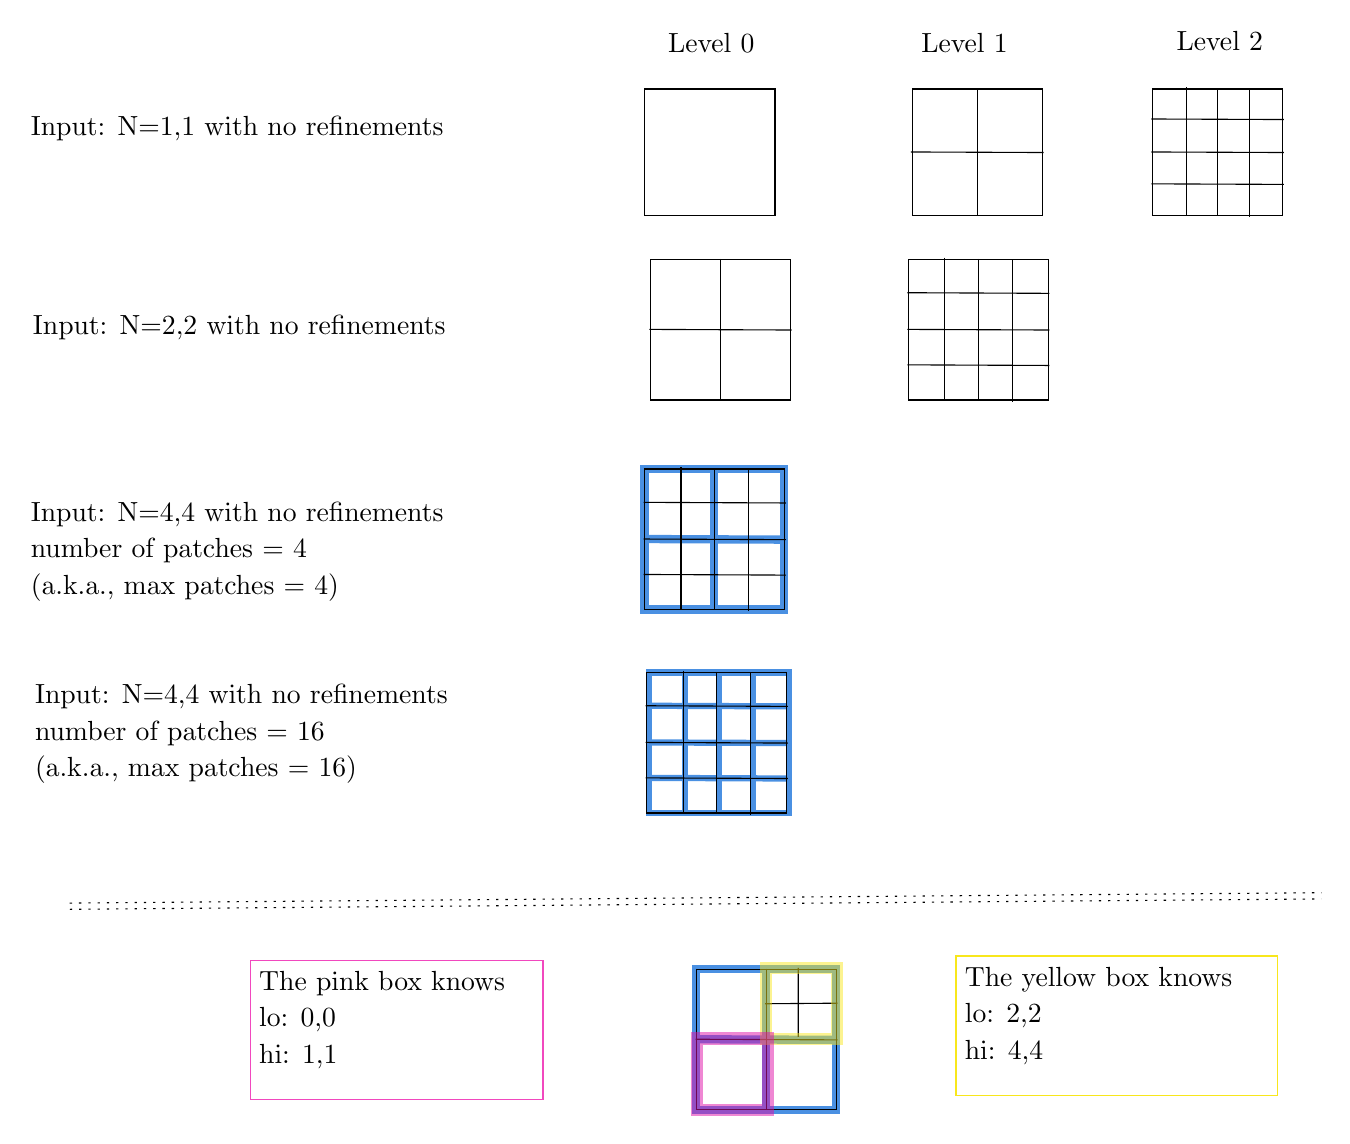
\begin{tikzpicture}[x=0.75pt,y=0.75pt,yscale=-1,xscale=1]
%uncomment if require: \path (0,581); %set diagram left start at 0, and has height of 581

%Shape: Rectangle [id:dp6371781385604116] 
\draw  [color={rgb, 255:red, 74; green, 144; blue, 226 }  ,draw opacity=1 ][line width=2.25]  (314.09,314.38) -- (381.42,314.38) -- (381.42,382.12) -- (314.09,382.12) -- cycle ;
%Straight Lines [id:da16828659063521467] 
\draw [color={rgb, 255:red, 74; green, 144; blue, 226 }  ,draw opacity=1 ][line width=2.25]    (347.75,314.09) -- (347.75,382.41) ;
%Straight Lines [id:da913893626068599] 
\draw [color={rgb, 255:red, 74; green, 144; blue, 226 }  ,draw opacity=1 ][line width=2.25]    (313.51,348.1) -- (382,348.4) ;
%Straight Lines [id:da7991985150003835] 
\draw [color={rgb, 255:red, 74; green, 144; blue, 226 }  ,draw opacity=1 ][line width=2.25]    (313.51,365.18) -- (382,365.48) ;
%Straight Lines [id:da1664140298792507] 
\draw [color={rgb, 255:red, 74; green, 144; blue, 226 }  ,draw opacity=1 ][line width=2.25]    (313.51,330.43) -- (382,330.73) ;
%Straight Lines [id:da3895198729400846] 
\draw [color={rgb, 255:red, 74; green, 144; blue, 226 }  ,draw opacity=1 ][line width=2.25]    (331.5,313.5) -- (331.5,381.82) ;
%Straight Lines [id:da7506315154110477] 
\draw [color={rgb, 255:red, 74; green, 144; blue, 226 }  ,draw opacity=1 ][line width=2.25]    (364.01,314.68) -- (364.01,383) ;

%Shape: Rectangle [id:dp5007081227877395] 
\draw   (312,33.29) -- (374.79,33.29) -- (374.79,94.21) -- (312,94.21) -- cycle ;
%Shape: Rectangle [id:dp18240877587778925] 
\draw   (440.83,33.29) -- (503.62,33.29) -- (503.62,94.21) -- (440.83,94.21) -- cycle ;
%Straight Lines [id:da6864437250811215] 
\draw    (472.22,33.03) -- (472.22,94.47) ;
%Straight Lines [id:da8988053086519276] 
\draw    (440.29,63.62) -- (504.16,63.88) ;

%Shape: Rectangle [id:dp7156491512427419] 
\draw   (556.67,33.29) -- (619.46,33.29) -- (619.46,94.21) -- (556.67,94.21) -- cycle ;
%Straight Lines [id:da2284438707437031] 
\draw    (588.06,33.03) -- (588.06,94.47) ;
%Straight Lines [id:da29012367457159915] 
\draw    (556.13,63.62) -- (620,63.88) ;
%Straight Lines [id:da06299977010030067] 
\draw    (556.13,78.98) -- (620,79.24) ;
%Straight Lines [id:da4842885889214601] 
\draw    (556.13,47.73) -- (620,47.99) ;
%Straight Lines [id:da04205672495045354] 
\draw    (572.91,32.5) -- (572.91,93.94) ;
%Straight Lines [id:da5186346722683335] 
\draw    (603.22,33.56) -- (603.22,95) ;


%Shape: Rectangle [id:dp06225261555233552] 
\draw   (314.87,115.38) -- (382.2,115.38) -- (382.2,183.12) -- (314.87,183.12) -- cycle ;
%Straight Lines [id:da5275983949406149] 
\draw    (348.54,115.09) -- (348.54,183.41) ;
%Straight Lines [id:da20200940747212215] 
\draw    (314.29,149.1) -- (382.78,149.4) ;

%Shape: Rectangle [id:dp6796803229454758] 
\draw   (439.09,115.38) -- (506.42,115.38) -- (506.42,183.12) -- (439.09,183.12) -- cycle ;
%Straight Lines [id:da16166756380911584] 
\draw    (472.75,115.09) -- (472.75,183.41) ;
%Straight Lines [id:da8256581238285523] 
\draw    (438.51,149.1) -- (507,149.4) ;
%Straight Lines [id:da7608690527075788] 
\draw    (438.51,166.18) -- (507,166.48) ;
%Straight Lines [id:da9831986325533246] 
\draw    (438.51,131.43) -- (507,131.73) ;
%Straight Lines [id:da7777810089283779] 
\draw    (456.5,114.5) -- (456.5,182.82) ;
%Straight Lines [id:da2355726961397997] 
\draw    (489.01,115.68) -- (489.01,184) ;


%Shape: Rectangle [id:dp8243447312549272] 
\draw  [color={rgb, 255:red, 74; green, 144; blue, 226 }  ,draw opacity=1 ][line width=3]  (311.87,216.38) -- (379.2,216.38) -- (379.2,284.12) -- (311.87,284.12) -- cycle ;
%Straight Lines [id:da7062001423638216] 
\draw [color={rgb, 255:red, 74; green, 144; blue, 226 }  ,draw opacity=1 ][line width=3]    (345.54,216.09) -- (345.54,284.41) ;
%Straight Lines [id:da0576109185320548] 
\draw [color={rgb, 255:red, 74; green, 144; blue, 226 }  ,draw opacity=1 ][line width=3]    (311.29,250.1) -- (379.78,250.4) ;

%Shape: Rectangle [id:dp3443685382901356] 
\draw   (312.09,216.38) -- (379.42,216.38) -- (379.42,284.12) -- (312.09,284.12) -- cycle ;
%Straight Lines [id:da6286683094563796] 
\draw    (345.75,216.09) -- (345.75,284.41) ;
%Straight Lines [id:da20004293878195178] 
\draw    (311.51,250.1) -- (380,250.4) ;
%Straight Lines [id:da04268522242507289] 
\draw    (311.51,267.18) -- (380,267.48) ;
%Straight Lines [id:da1201188746406956] 
\draw    (311.51,232.43) -- (380,232.73) ;
%Straight Lines [id:da43066817262520085] 
\draw    (329.5,215.5) -- (329.5,283.82) ;
%Straight Lines [id:da6580735263266981] 
\draw    (362.01,216.68) -- (362.01,285) ;


%Shape: Rectangle [id:dp8119746351867834] 
\draw   (313.09,314.38) -- (380.42,314.38) -- (380.42,382.12) -- (313.09,382.12) -- cycle ;
%Straight Lines [id:da7445678895475916] 
\draw    (346.75,314.09) -- (346.75,382.41) ;
%Straight Lines [id:da41632760867261087] 
\draw    (312.51,348.1) -- (381,348.4) ;
%Straight Lines [id:da21592424963972423] 
\draw    (312.51,365.18) -- (381,365.48) ;
%Straight Lines [id:da8698160068576049] 
\draw    (312.51,330.43) -- (381,330.73) ;
%Straight Lines [id:da34366175442266544] 
\draw    (330.5,313.5) -- (330.5,381.82) ;
%Straight Lines [id:da6765418222201485] 
\draw    (363.01,314.68) -- (363.01,383) ;

%Straight Lines [id:da21257546822462925] 
\draw  [dash pattern={on 0.84pt off 2.51pt}]  (34.99,425.5) -- (637.99,420.5)(35.01,428.5) -- (638.01,423.5) ;
%Shape: Rectangle [id:dp26141148832467387] 
\draw  [color={rgb, 255:red, 74; green, 144; blue, 226 }  ,draw opacity=1 ][line width=3]  (336.87,457.38) -- (404.2,457.38) -- (404.2,525.12) -- (336.87,525.12) -- cycle ;
%Straight Lines [id:da2970415252540526] 
\draw [color={rgb, 255:red, 74; green, 144; blue, 226 }  ,draw opacity=1 ][line width=3]    (370.54,457.09) -- (370.54,525.41) ;
%Straight Lines [id:da3811766428224914] 
\draw [color={rgb, 255:red, 74; green, 144; blue, 226 }  ,draw opacity=1 ][line width=3]    (336.29,491.1) -- (404.78,491.4) ;

%Shape: Rectangle [id:dp2597434048703462] 
\draw   (337.09,457.38) -- (404.42,457.38) -- (404.42,525.12) -- (337.09,525.12) -- cycle ;
%Straight Lines [id:da8210500912108043] 
\draw    (370.75,457.09) -- (370.75,525.41) ;
%Straight Lines [id:da6553054114566375] 
\draw    (336.51,491.1) -- (405,491.4) ;
%Straight Lines [id:da49874604231381214] 
\draw    (370,474) -- (405,473.73) ;
%Straight Lines [id:da32155055284696665] 
\draw    (386.01,456.68) -- (386,490) ;

%Shape: Rectangle [id:dp00564518741570641] 
\draw  [color={rgb, 255:red, 248; green, 231; blue, 28 }  ,draw opacity=0.49 ][line width=4.5]  (370.38,456.71) -- (404.62,456.71) -- (404.62,491.02) -- (370.38,491.02) -- cycle ;
%Shape: Rectangle [id:dp5478244264394843] 
\draw  [color={rgb, 255:red, 224; green, 16; blue, 168 }  ,draw opacity=0.5 ][line width=4.5]  (337.09,490.81) -- (371.33,490.81) -- (371.33,525.12) -- (337.09,525.12) -- cycle ;


% Text Node
\draw (15,45) node [anchor=north west][inner sep=0.75pt]   [align=left] {Input: N=1,1 with no refinements};
% Text Node
\draw (444,5) node [anchor=north west][inner sep=0.75pt]   [align=left] {Level 1};
% Text Node
\draw (567,4) node [anchor=north west][inner sep=0.75pt]   [align=left] {Level 2};
% Text Node
\draw (322,5) node [anchor=north west][inner sep=0.75pt]   [align=left] {Level 0};
% Text Node
\draw (16,141) node [anchor=north west][inner sep=0.75pt]   [align=left] {Input: N=2,2 with no refinements};
% Text Node
\draw (15,231) node [anchor=north west][inner sep=0.75pt]   [align=left] {Input: N=4,4 with no refinements\\number of patches = 4\\(a.k.a., max patches = 4)};
% Text Node
\draw (17,319) node [anchor=north west][inner sep=0.75pt]   [align=left] {Input: N=4,4 with no refinements\\number of patches = 16\\(a.k.a., max patches = 16)};
% Text Node
\draw  [color={rgb, 255:red, 248; green, 231; blue, 28 }  ,draw opacity=1 ]  (462,451) -- (617,451) -- (617,518) -- (462,518) -- cycle  ;
\draw (465,455) node [anchor=north west][inner sep=0.75pt]   [align=left] {The yellow box knows\\lo: 2,2\\hi: 4,4};
% Text Node
\draw  [color={rgb, 255:red, 237; green, 21; blue, 172 }  ,draw opacity=0.78 ]  (122,453) -- (263,453) -- (263,520) -- (122,520) -- cycle  ;
\draw (125,457) node [anchor=north west][inner sep=0.75pt]   [align=left] {The pink box knows\\lo: 0,0\\hi: 1,1};

\end{tikzpicture}


\section{Time loop in IBAMR}
This is simply done by: 
\begin{itemize}
    \item use IntegrateHierarchy, IBIntegrateHierarchy, IBExplicitIntegrateHierarchy, etc;
    \item do a loop in time;
    \item call advanceHierarchy(dt);
\end{itemize}

\section{Boundary conditions in IBAMR}
General periodic boundary conditions can be imposed using the input file. 
 See \href{https://02313823769317816526.googlegroups.com/attach/587d96cc21b52/boundary_conditions.pdf?part=0.1&view=1&vt=ANaJVrF8UYShkZrnq_l7gR-MAsURdgZ_sh2IHjGJpdAz2yKdK7PcnZhHPHmkhwHbT59R_wDEtnOB74swxRhnIme17Z6ca5gqZFrGBX3J8vX2-HmB1jQ491A}{this document by Aaron Barret}.

\section{Stability, Consistency, and Convergence}
Consider the second order ode with known boundary conditions: $$u''=f$$% with given boundary conditions. 

Start with a Finite Difference method: $$\frac{U_{i+1}-2U_i+U_{i-1}}{h^2} = f_i$$

Want to show that with a second order stencil $||E||_2 = \mathcal{O}(h^2)$. Where $E = U - \hat{U}$.

Local truncation error: define $\tau$ by substituting the true solution into the difference equation and substituting the taylor expansion of u into the result
$$\tau = \frac{u_{i+1}-2u_i+u_{i-1}}{h^2} - f_i = h^2u''+\mathcal{O}(h^4)$$

Now we define the global error. Let $U$ be the true solution and $\hat{U}$ be the approximated solution. So $AU=F$ and $A\hat{U}=F+\tau$, where $A$ is the second derivative operator. Then define $E=U-\hat{U}$. With this we have $AE=-\tau$ which corresponds to the differential equation $$e''=-\tau$$Substituting $\tau$ in and integrating twice, we get the solution $$e=-h^2u+\mathcal{O}(h^4)=\mathcal{O}(h^2).$$

To determine stability, consider the discrete form of the differential equation for the global error. $$A^hE^h=-\tau^h$$
From this we have
$$||E^h|| \leq ||(A^h)^{-1}||||\tau^h||$$
Since $||\tau^h|| = \mathcal{O}(h^2)$, we can bound the error by bounding the remaining norm. 

\subsection{Stability}
A system is stable if there exists a constant $C$ so that $$||(A^h)^{-1}|| \leq C,\quad \text{as}\quad h\to 0$$

\subsection{Consistency}
A system is consistent if $$||\tau^h||\to 0 \quad \text{as} \quad h\to 0$$

\subsection{Convergence}
A method is convergent if $$||E^h|| \to 0 \quad \text{as} \quad h\to 0$$
or equivalently if it is stable and consistent.


\section{QUESTIONS}

\begin{itemize}
    \item  User Guide - page 18 - whu 19,5 and not 19,6?
    \item Patch How does a know the ghost width without knowing $\Delta x$? 
    it's 0,1,2 or 3 or whatever. It is just the number of cells in each direction
\end{itemize}

\section{General concepts}
When running an IBAMR example, we will have input files (usually called input2d, input3d). There you can define variables for multiple classes and functions. 
The source codes will have access to such information by using {\color{red} getContextData -check this} 

\subsection{Collocated strategy}

\subsection{Staggered strategy}
Usually the one used for solving incompressible navier stokes

\subsection{Contexts}
IBAMR has $3$ contexts: current\_data, new\_data and scratch\_data. It also includes unknown\_variable\_context\_type. 
As you can see, some of them are related to time. 

The scratch includes the ghosts values:

\tikzset{every picture/.style={line width=0.75pt}} %set default line width to 0.75pt        

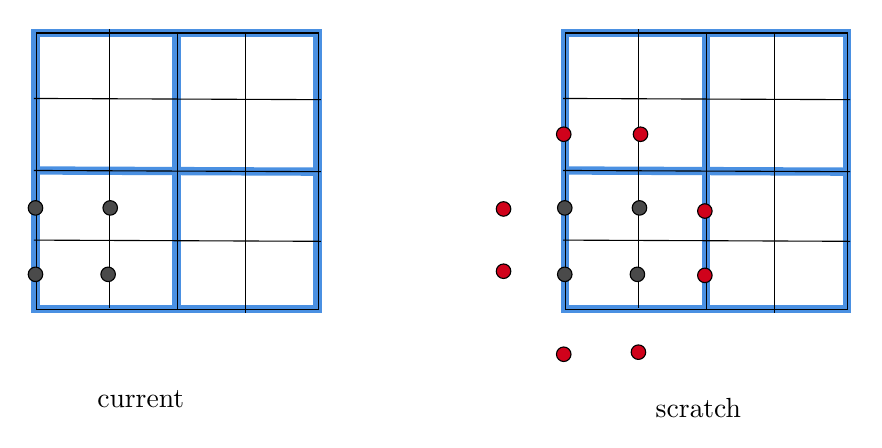
\begin{tikzpicture}[x=0.75pt,y=0.75pt,yscale=-1,xscale=1]
%uncomment if require: \path (0,300); %set diagram left start at 0, and has height of 300

%Shape: Rectangle [id:dp17462798752095665] 
\draw  [color={rgb, 255:red, 74; green, 144; blue, 226 }  ,draw opacity=1 ][line width=3]  (367.46,36.24) -- (503.39,36.24) -- (503.39,169.26) -- (367.46,169.26) -- cycle ;
%Straight Lines [id:da17434761539112165] 
\draw [color={rgb, 255:red, 74; green, 144; blue, 226 }  ,draw opacity=1 ][line width=3]    (435.42,35.66) -- (435.42,169.84) ;
%Straight Lines [id:da4733491508432628] 
\draw [color={rgb, 255:red, 74; green, 144; blue, 226 }  ,draw opacity=1 ][line width=3]    (366.29,102.46) -- (504.56,103.04) ;

%Shape: Rectangle [id:dp11075672832714578] 
\draw   (367.9,36.24) -- (503.83,36.24) -- (503.83,169.26) -- (367.9,169.26) -- cycle ;
%Straight Lines [id:da6379417313736702] 
\draw    (435.86,35.66) -- (435.86,169.84) ;
%Straight Lines [id:da8324515121375866] 
\draw    (366.73,102.46) -- (505,103.04) ;
%Straight Lines [id:da1772969193566729] 
\draw    (366.73,136.01) -- (505,136.59) ;
%Straight Lines [id:da9597797458054791] 
\draw    (366.73,67.76) -- (505,68.34) ;
%Straight Lines [id:da262849999412053] 
\draw    (403.05,34.5) -- (403.05,168.69) ;
%Straight Lines [id:da05811246862536157] 
\draw    (468.67,36.81) -- (468.67,171) ;


%Shape: Circle [id:dp35861085270045456] 
\draw  [fill={rgb, 255:red, 74; green, 74; blue, 74 }  ,fill opacity=1 ] (364,120.5) .. controls (364,118.57) and (365.57,117) .. (367.5,117) .. controls (369.43,117) and (371,118.57) .. (371,120.5) .. controls (371,122.43) and (369.43,124) .. (367.5,124) .. controls (365.57,124) and (364,122.43) .. (364,120.5) -- cycle ;
%Shape: Circle [id:dp5135567978588242] 
\draw  [fill={rgb, 255:red, 74; green, 74; blue, 74 }  ,fill opacity=1 ] (400,120.5) .. controls (400,118.57) and (401.57,117) .. (403.5,117) .. controls (405.43,117) and (407,118.57) .. (407,120.5) .. controls (407,122.43) and (405.43,124) .. (403.5,124) .. controls (401.57,124) and (400,122.43) .. (400,120.5) -- cycle ;
%Shape: Circle [id:dp6938347114097798] 
\draw  [fill={rgb, 255:red, 74; green, 74; blue, 74 }  ,fill opacity=1 ] (399,152.5) .. controls (399,150.57) and (400.57,149) .. (402.5,149) .. controls (404.43,149) and (406,150.57) .. (406,152.5) .. controls (406,154.43) and (404.43,156) .. (402.5,156) .. controls (400.57,156) and (399,154.43) .. (399,152.5) -- cycle ;
%Shape: Circle [id:dp15593112495174166] 
\draw  [fill={rgb, 255:red, 74; green, 74; blue, 74 }  ,fill opacity=1 ] (364,152.5) .. controls (364,150.57) and (365.57,149) .. (367.5,149) .. controls (369.43,149) and (371,150.57) .. (371,152.5) .. controls (371,154.43) and (369.43,156) .. (367.5,156) .. controls (365.57,156) and (364,154.43) .. (364,152.5) -- cycle ;
%Shape: Circle [id:dp9736844819109725] 
\draw  [fill={rgb, 255:red, 208; green, 2; blue, 27 }  ,fill opacity=1 ] (363.5,85) .. controls (363.5,83.07) and (365.07,81.5) .. (367,81.5) .. controls (368.93,81.5) and (370.5,83.07) .. (370.5,85) .. controls (370.5,86.93) and (368.93,88.5) .. (367,88.5) .. controls (365.07,88.5) and (363.5,86.93) .. (363.5,85) -- cycle ;
%Shape: Circle [id:dp036710362790118634] 
\draw  [fill={rgb, 255:red, 208; green, 2; blue, 27 }  ,fill opacity=1 ] (400.5,85) .. controls (400.5,83.07) and (402.07,81.5) .. (404,81.5) .. controls (405.93,81.5) and (407.5,83.07) .. (407.5,85) .. controls (407.5,86.93) and (405.93,88.5) .. (404,88.5) .. controls (402.07,88.5) and (400.5,86.93) .. (400.5,85) -- cycle ;
%Shape: Circle [id:dp3173520123149851] 
\draw  [fill={rgb, 255:red, 208; green, 2; blue, 27 }  ,fill opacity=1 ] (334.5,121) .. controls (334.5,119.07) and (336.07,117.5) .. (338,117.5) .. controls (339.93,117.5) and (341.5,119.07) .. (341.5,121) .. controls (341.5,122.93) and (339.93,124.5) .. (338,124.5) .. controls (336.07,124.5) and (334.5,122.93) .. (334.5,121) -- cycle ;
%Shape: Circle [id:dp20141904604722072] 
\draw  [fill={rgb, 255:red, 208; green, 2; blue, 27 }  ,fill opacity=1 ] (334.5,151) .. controls (334.5,149.07) and (336.07,147.5) .. (338,147.5) .. controls (339.93,147.5) and (341.5,149.07) .. (341.5,151) .. controls (341.5,152.93) and (339.93,154.5) .. (338,154.5) .. controls (336.07,154.5) and (334.5,152.93) .. (334.5,151) -- cycle ;
%Shape: Circle [id:dp8105588765705645] 
\draw  [fill={rgb, 255:red, 208; green, 2; blue, 27 }  ,fill opacity=1 ] (363.5,191) .. controls (363.5,189.07) and (365.07,187.5) .. (367,187.5) .. controls (368.93,187.5) and (370.5,189.07) .. (370.5,191) .. controls (370.5,192.93) and (368.93,194.5) .. (367,194.5) .. controls (365.07,194.5) and (363.5,192.93) .. (363.5,191) -- cycle ;
%Shape: Circle [id:dp7044675686765425] 
\draw  [fill={rgb, 255:red, 208; green, 2; blue, 27 }  ,fill opacity=1 ] (399.5,190) .. controls (399.5,188.07) and (401.07,186.5) .. (403,186.5) .. controls (404.93,186.5) and (406.5,188.07) .. (406.5,190) .. controls (406.5,191.93) and (404.93,193.5) .. (403,193.5) .. controls (401.07,193.5) and (399.5,191.93) .. (399.5,190) -- cycle ;
%Shape: Circle [id:dp39772774187159277] 
\draw  [fill={rgb, 255:red, 208; green, 2; blue, 27 }  ,fill opacity=1 ] (431.5,122) .. controls (431.5,120.07) and (433.07,118.5) .. (435,118.5) .. controls (436.93,118.5) and (438.5,120.07) .. (438.5,122) .. controls (438.5,123.93) and (436.93,125.5) .. (435,125.5) .. controls (433.07,125.5) and (431.5,123.93) .. (431.5,122) -- cycle ;
%Shape: Circle [id:dp445786909946031] 
\draw  [fill={rgb, 255:red, 208; green, 2; blue, 27 }  ,fill opacity=1 ] (431.5,153) .. controls (431.5,151.07) and (433.07,149.5) .. (435,149.5) .. controls (436.93,149.5) and (438.5,151.07) .. (438.5,153) .. controls (438.5,154.93) and (436.93,156.5) .. (435,156.5) .. controls (433.07,156.5) and (431.5,154.93) .. (431.5,153) -- cycle ;

%Shape: Rectangle [id:dp5892434006525284] 
\draw  [color={rgb, 255:red, 74; green, 144; blue, 226 }  ,draw opacity=1 ][line width=3]  (112.46,36.24) -- (248.39,36.24) -- (248.39,169.26) -- (112.46,169.26) -- cycle ;
%Straight Lines [id:da7691092198996545] 
\draw [color={rgb, 255:red, 74; green, 144; blue, 226 }  ,draw opacity=1 ][line width=3]    (180.42,35.66) -- (180.42,169.84) ;
%Straight Lines [id:da8058570159782643] 
\draw [color={rgb, 255:red, 74; green, 144; blue, 226 }  ,draw opacity=1 ][line width=3]    (111.29,102.46) -- (249.56,103.04) ;

%Shape: Rectangle [id:dp2074491181786935] 
\draw   (112.9,36.24) -- (248.83,36.24) -- (248.83,169.26) -- (112.9,169.26) -- cycle ;
%Straight Lines [id:da9433141248982548] 
\draw    (180.86,35.66) -- (180.86,169.84) ;
%Straight Lines [id:da40022499955953483] 
\draw    (111.73,102.46) -- (250,103.04) ;
%Straight Lines [id:da6723261154656262] 
\draw    (111.73,136.01) -- (250,136.59) ;
%Straight Lines [id:da8148261434119071] 
\draw    (111.73,67.76) -- (250,68.34) ;
%Straight Lines [id:da8309638091592957] 
\draw    (148.05,34.5) -- (148.05,168.69) ;
%Straight Lines [id:da6197070602927712] 
\draw    (213.67,36.81) -- (213.67,171) ;


%Shape: Circle [id:dp24610059946874419] 
\draw  [fill={rgb, 255:red, 74; green, 74; blue, 74 }  ,fill opacity=1 ] (109,120.5) .. controls (109,118.57) and (110.57,117) .. (112.5,117) .. controls (114.43,117) and (116,118.57) .. (116,120.5) .. controls (116,122.43) and (114.43,124) .. (112.5,124) .. controls (110.57,124) and (109,122.43) .. (109,120.5) -- cycle ;
%Shape: Circle [id:dp6643879468036364] 
\draw  [fill={rgb, 255:red, 74; green, 74; blue, 74 }  ,fill opacity=1 ] (145,120.5) .. controls (145,118.57) and (146.57,117) .. (148.5,117) .. controls (150.43,117) and (152,118.57) .. (152,120.5) .. controls (152,122.43) and (150.43,124) .. (148.5,124) .. controls (146.57,124) and (145,122.43) .. (145,120.5) -- cycle ;
%Shape: Circle [id:dp05578966222918358] 
\draw  [fill={rgb, 255:red, 74; green, 74; blue, 74 }  ,fill opacity=1 ] (144,152.5) .. controls (144,150.57) and (145.57,149) .. (147.5,149) .. controls (149.43,149) and (151,150.57) .. (151,152.5) .. controls (151,154.43) and (149.43,156) .. (147.5,156) .. controls (145.57,156) and (144,154.43) .. (144,152.5) -- cycle ;
%Shape: Circle [id:dp2067799049886656] 
\draw  [fill={rgb, 255:red, 74; green, 74; blue, 74 }  ,fill opacity=1 ] (109,152.5) .. controls (109,150.57) and (110.57,149) .. (112.5,149) .. controls (114.43,149) and (116,150.57) .. (116,152.5) .. controls (116,154.43) and (114.43,156) .. (112.5,156) .. controls (110.57,156) and (109,154.43) .. (109,152.5) -- cycle ;

% Text Node
\draw (141,207) node [anchor=north west][inner sep=0.75pt]   [align=left] {current };
% Text Node
\draw (410,211) node [anchor=north west][inner sep=0.75pt]   [align=left] {scratch};


\end{tikzpicture}

\subsection{Tagging method}
This will be the method used to decide if the patch should be refined or not, and how much refinement we need. 
Essentially it will use the parameters minref ..., maxref to define this. 


{\color{red} include examples from pictures here}

\paragraph{GradientDetector}
Decides where to refine the grid. 

tagged cells -> error detector


\section{Immersed Boundary Concepts}
\subsection{MFAC}
Ratio of fluid cell width to solid cell width. Good choices for MFAC avoid leaks

Section 2.5 of this paper
\url{https://arxiv.org/pdf/2105.14536.pdf}

Specify cell width for fluid (Eulerian grid) and then use MFAC to determine cell width for solid (Lagrangian)

\section{Examples IBAMR}
\subsection{Visualizing in VisIt}
If the physical coordinates and material coordinates coincide initially, then displacing the mesh by $dX$ will show us the initial position of the solid.
Notice that for ex0, the \texttt{registerInitialCoordinateMappingFunction} transforms a slab into a circular band. See figure   

\begin{figure}[H]
    \begin{subfigure}[b]{0.45\textwidth}
         \centering
        \includegraphics[width=\textwidth]{viz_mesh.png}
         \end{subfigure}
     \hfill
     \begin{subfigure}[b]{0.45\textwidth}
     \centering
    \includegraphics[width=\textwidth]{vix_mesh_displace.png}
     \end{subfigure}
     \caption{How to visualize mesh displacement by $dX$ in ex0.}
\end{figure}

\subsection{IBFE/explicit/ex0}

Uses periodic boundary conditions

\subsection{IBFE/explicit/ex1}

Uses periodic boundary conditions


\section{List of abbreviations and common terms}
\begin{itemize}
    \item MAC - marker and cell
    \item CC - cell centered
    \item SC - side centered
    \item IBTK - Immersed Boundary Toolkit
\end{itemize}


\section*{References}
[1] Anderson, R., Arrighi, W., Elliott, N., Gunney, B., \& Hornung, R. (2013). SAMRAI concepts and software design. Lawrence Livermore Nat. Lab. Rept. LLNL-SM-617092-DRAFT.

\end{document}      